\documentclass[AMA,STIX2COL,Linenumberson]{MRM}
\articletype{Research Article}%

\topskip=0pt
\raggedbottom

%% ---------------------------------------------------------------------------
%% Draft scaffolding. Remove \DRAFTtrue before submission to hide all markers.
%% ---------------------------------------------------------------------------
\usepackage{xcolor}
\newif\ifDRAFT
\DRAFTtrue
\ifDRAFT
  \newcommand{\TODO}[1]{{\color{red}\textbf{[TODO: #1]}}}
  \newcommand{\NUM}[1]{{\color{red}\textbf{[#1]}}}
  \newcommand{\NOTE}[1]{{\color{blue}\small\textit{[note: #1]}}}
\else
  \newcommand{\TODO}[1]{}
  \newcommand{\NUM}[1]{#1}
  \newcommand{\NOTE}[1]{}
\fi

%% Workaround for a bug in MRM.cls: when the abstract is too tall for the title
%% page the class splits it and references \@firstpage@foot@height, which it never
%% defines. Harmless when the abstract does fit.
\makeatletter
\@ifundefined{@firstpage@foot@height}{%
  \newdimen\@firstpage@foot@height \@firstpage@foot@height=0pt}{}
\makeatother

%% Placeholder figure box so the draft compiles before the artwork exists.
\newcommand{\figplaceholder}[2]{%
  \fbox{\parbox[c][#2][c]{0.98\linewidth}{\centering\color{gray}\small #1}}}

\begin{document}

%% Alternative titles considered:
%%   "Fibre orientation from the signal, not from diffusion: hollow-cylinder
%%    $\chi$-separation of paramagnetic and diamagnetic susceptibility"
%%    -- rejected: overstates the role of $\theta$, which never enters the separation.
%%   "$R_2'$-anchored hollow-cylinder fitting of the multi-echo gradient-echo magnitude"
\title{Susceptibility source separation with white-matter fibre orientation and myelin water fraction recovered from the gradient-echo magnitude}

\author[1,2]{Ashley W. Stewart}
%% \TODO{co-authors}: add \author[n]{Name} lines here (no \TODO inside \author --- it is a moving argument)

\authormark{Stewart \textsc{et al}}

\address[1]{\orgdiv{School of Electrical Engineering and Computer Science}, \orgname{The University of Queensland}, \orgaddress{\state{Brisbane, Queensland}, \country{Australia}}}
\address[2]{\orgdiv{Centre for Advanced Imaging}, \orgname{The University of Queensland}, \orgaddress{\state{Brisbane, Queensland}, \country{Australia}}}

\corres{Ashley Stewart, \email{ashley.stewart@uq.edu.au}}

\finfo{\TODO{funding statement}}

%% MRM allows 250 words for a structured abstract. Re-check after the two in vivo
%% sentences are added.
\abstract[Summary]{
\section{Purpose}
Susceptibility source separation is under-determined in white matter because the relaxivity linking susceptibility to reversible relaxation depends on the fibre-to-$B_0$ angle $\theta$, which single-orientation data cannot see. We show that $\theta$ and the myelin water fraction (MWF) are recoverable from the multi-echo gradient-echo (GRE) magnitude already acquired for quantitative susceptibility mapping, provided the fit is anchored to the measured reversible rate $R_2'$.

\section{Methods}
Myelinated white matter is modelled as three water pools---myelin, axonal, extra-axonal---whose orientation-dependent frequency offsets (Wharton--Bowtell hollow-cylinder model) make the magnitude decay non-mono-exponential in a $\theta$- and MWF-dependent way. The resulting fit is uniquely identifiable but ill-conditioned along a $\theta$/decay-rate trade-off valley; anchoring the total reversible rate to the measured $R_2'$ collapses it. White matter is located by model selection against a mono-exponential alternative. The recovered parameters then drive the separation: the conventional closed-form solve outside white matter, a myelin-content route inside it. The method runs end to end on a QSM, an $R_2'$ map and the magnitude, with no segmentation, atlas or diffusion input. Evaluation used the QSM-CI benchmark against held-out ground truth and \TODO{in vivo cohort, one line}.

\section{Results}
Anchoring improved fibre-angle estimation from a correlation of 0.72 (median absolute error $10.6^\circ$) to 0.86 ($8.4^\circ$), and MWF from 0.29 to 0.81 (0.015). White matter was located at Dice 0.893 against a held-out label. Separation reached 24.6\,\% average detrended NRMSE against 43.4\,\% for the closed-form null solution, 46.1\,\% for SUSEP-Net and 78.1\,\% for $\chi$-sepnet; pinning $\theta$ to the ground-truth fibre angle did not improve on the signal-derived estimate (25.7 vs 24.6\,\%). \TODO{one sentence of in vivo result}

\section{Conclusion}
Fibre orientation and myelin water fraction can be estimated at 7\,T from data already acquired for QSM. Orientation acts not as a correction applied to the separation---it enters neither branch---but as the nuisance parameter that must be resolved before MWF becomes identifiable. The white-matter separation inherits one calibration, the constant converting MWF to susceptibility, which in vivo data rather than a matched phantom must test.
}

\keywords{quantitative susceptibility mapping, susceptibility source separation, $\chi$-separation, myelin, white matter microstructure, fibre orientation, hollow cylinder model}

\maketitle


%% ===========================================================================
\section{Introduction}
%% ===========================================================================

Magnetic susceptibility measured by QSM is a signed sum of contributions of opposite sign \cite{schweser_foundations_2016,haacke_quantitative_2015}. Iron, stored predominantly as ferritin and haemosiderin, is paramagnetic; myelin lipids and calcium are diamagnetic \cite{duyn_contributions_2017,liu_susceptibilityweighted_2015}. In tissues where the two coexist---white matter and the iron-rich deep grey nuclei above all---a single susceptibility value cannot distinguish a voxel with little of either from a voxel in which large opposing contributions have cancelled. This matters clinically wherever iron accumulation and demyelination occur together, as in multiple sclerosis lesions \cite{kiersnowski_investigating_2023} and in neurodegeneration \cite{langkammer_quantitative_2018,wisnieff_quantitative_2015}, and it is the reason susceptibility source separation exists.

The standard resolution is to add a second, additively combining measurement. In the static-dephasing regime, reversible transverse relaxation is driven by the magnitude of the local field perturbation rather than its sign \cite{yablonskiy_theory_1994}, so paramagnetic and diamagnetic sources both increase $R_2' = R_2^{*} - R_2$ while they subtract in $\chi$. Two measurements and two unknowns give a determined system, linked by the relaxivity $D_r$ that converts susceptibility into reversible dephasing rate. This is the skeleton shared by every current source-separation method, whether the solve is closed-form and regularised, as in $\chi$-separation \cite{shin_chiseparation_2021} and WaveSep \cite{fang_wavesep_2023}, performed in the signal domain, as in DECOMPOSE \cite{chen_decompose_2021} and APART-QSM \cite{apartqsm_TODO}, based on magnitude decay modelling alone \cite{dimov_r2star_2022}, or learned \cite{kim_chisepnet_2025,susepnet_TODO}.

The difficulty is that $D_r$ is not a material constant but a description of microstructure. In the static-dephasing derivation the relaxivity is set by the geometry of the perturbing inclusions: randomly distributed spherical sources give an isotropic $D_r^{+} = 2\pi\bar\gamma B_0/(9\sqrt{3})$, whereas parallel cylinders---the geometry of myelinated axons---give $D_r^{-}(\theta) = \tfrac{1}{2}\bar\gamma B_0 \sin^2\theta$, vanishing for fibres aligned with $B_0$ \cite{yablonskiy_theory_1994,brown_distribution_1961}. The second equation therefore contains a third unknown, the fibre-to-$B_0$ angle, and the system is under-determined once more. The problem compounds because the diamagnetic susceptibility of white matter is itself anisotropic, $\chi^{-}(\theta) = (\chi_{\parallel}-\chi_{\perp})\cos^{2}\theta + \chi^{-}_{\mathrm{iso}}$. Ridani et al.\ \cite{ridani_realistic_2026} recently quantified the consequence and found orientation-induced error to be a dominant systematic error of white-matter source separation.

Existing methods dispose of $\theta$ in one of four ways, each with a cost. The most common is to assume it away, applying a single empirical scalar relaxivity---137\,Hz/ppm in $\chi$-separation \cite{shin_chiseparation_2021}, 114\,Hz/ppm in the $\chi$-sepnet calibration \cite{kim_chisepnet_2025}---obtained by regressing $R_2'$ against QSM in iron-rich deep grey nuclei, where the sources are spherical, and then applying it to myelin cylinders, where they are not. The result is a systematic, orientation-patterned white-matter bias, and, as we show below, brittleness: a network with the calibration baked in degrades from competitive to worst-in-class when the relaxivity scale of the data moves. The second option is to buy the angle with a diffusion acquisition, taking $\theta$ from the principal eigenvector of a DTI fit. This costs scan time, requires an accurate cross-modality registration, and assumes a single fibre population per voxel. The third is to buy it with head rotation, acquiring at multiple orientations, which is impractical in the clinic. The fourth is to learn the mapping and let a network marginalise the angle implicitly, which works within the training distribution and fails silently outside it.

The observation this work is built on is that the microstructure responsible for the orientation dependence of $D_r^{-}$ also leaves a second, independent trace in data that source-separation methods already acquire. A myelinated voxel is not a single water pool but at least three---myelin water trapped between the sheath bilayers, intra-axonal water, and extra-axonal water---and the anisotropic, radially oriented susceptibility of the sheath places these pools at different Larmor frequencies, with offsets that depend on $\theta$ through the hollow-cylinder field of an infinite myelinated axon \cite{wharton_fiber_2012,wharton_gradient_2013,sukstanskii_role_2014}. The pools interfere, and the multi-echo GRE magnitude is consequently not mono-exponential: its \emph{shape} carries $\theta$ and the myelin water fraction. One mechanism, two observable consequences---an orientation-dependent relaxivity and an orientation-dependent decay shape---and the second is measurable from data that a source-separation study already acquires. What the decay shape delivers is a pair of microstructural parameters, the fibre angle and the myelin water fraction; we treat the recovery of that pair as the primary problem, and source separation as one application of it.

Two obstacles explain why this has not simply been done, and both are quantified here. The first is amplitude. The pool frequency offsets scale with $B_0$, and at typical clinical field the interference is small relative to noise: in the field study reported below, $\theta$ is essentially unrecoverable at 1.27\,T (median error $25^\circ$, against roughly $30^\circ$ for a random guess over $[0^\circ,90^\circ]$), marginal at 3\,T ($10^\circ$) and well recovered at 7\,T ($3^\circ$). This work is therefore, in its present form, a high-field method, and we state that scope at the outset. The second obstacle is conditioning. Even where the interference is visible, the per-voxel estimation problem---although uniquely identifiable in the noiseless limit---has its minimum at the bottom of a long, shallow, curved valley in which a larger fibre angle trades against a smaller mesoscopic dephasing rate, since both increase the net decay and only the non-mono-exponential curvature distinguishes them. At the effective white-matter SNR of a realistic acquisition, per-voxel myelin-water-fraction and rate estimates fall at or beyond the anatomical spread of those parameters; the fit is noise-limited rather than resolution-limited, and refining the search grid changes nothing.

Our resolution is that the quantity along which the valley runs, the total reversible decay rate, is exactly the quantity that has already been measured. Requiring the model's own analytic reversible rate, plus a non-negative mesoscopic remainder, to equal the observed $R_2'$ removes the ill-conditioned direction and turns a noise-limited three-parameter fit into a well-conditioned two-parameter one. This paper contributes: (i) an $R_2'$-anchored hollow-cylinder estimator of fibre orientation and myelin water fraction from single-orientation multi-echo GRE magnitude, with an identifiability and conditioning analysis establishing the acquisition regime in which it can work; (ii) a model-selection rule that locates myelinated white matter from the data alone, with no segmentation input; (iii) a complete source-separation method built on them, requiring no segmentation, atlas or diffusion input, in which the solve outside white matter is the conventional closed form and the white-matter solve is routed through the myelin water fraction, evaluated on a public benchmark with held-out ground truth against the closed-form null solution and learned comparators; and \TODO{(iv) in vivo demonstration --- write once the cohort is fixed}.


%% ===========================================================================
\section{Theory}
%% ===========================================================================

\subsection{The under-determined voxel and the relaxometric second equation}

Within a voxel, the measured susceptibility is the sum of a paramagnetic and a diamagnetic contribution,
\begin{equation}
\chi_{\mathrm{total}} = \chi^{+} + \chi^{-}, \qquad \chi^{+} \ge 0 \ge \chi^{-},
\label{eq:sum}
\end{equation}
which is one equation in two unknowns. Throughout this paper $\chi^{-}$ is reported as a signed, non-positive quantity; the benchmark stores it as a positive magnitude, and we negate where required for scoring.

In the static-dephasing regime, reversible relaxation depends on $|\Delta\omega|$ and the two source types therefore add \cite{yablonskiy_theory_1994}:
\begin{equation}
R_2' \;=\; R_2^{*} - R_2 \;=\; D_r^{+}\,|\chi^{+}| \;+\; D_r^{-}\,|\chi^{-}| .
\label{eq:r2p}
\end{equation}
Equations~\eqref{eq:sum} and~\eqref{eq:r2p} form a $2\times2$ linear system with solution
\begin{equation}
\chi^{+} = \frac{R_2' + D_r^{-}\chi_{\mathrm{total}}}{D_r^{+}+D_r^{-}}, \qquad
|\chi^{-}| = \frac{R_2' - D_r^{+}\chi_{\mathrm{total}}}{D_r^{+}+D_r^{-}},
\label{eq:solve}
\end{equation}
which for a single relaxivity $D_r^{+}=D_r^{-}=D_r$ reduces to
\begin{equation}
\chi^{\pm} = \tfrac{1}{2}\left(\chi_{\mathrm{total}} \pm R_2'/D_r\right).
\label{eq:null}
\end{equation}
Equation~\eqref{eq:null} is worth stating plainly, because it defines what is and is not difficult about source separation: when $D_r$ is a known constant, the problem is algebraically determined and everything else in the literature is regularisation, noise handling, or the recovery of $\chi_{\mathrm{total}}$ and $R_2'$ themselves. We use \eqref{eq:null} as a scored null baseline throughout.

\subsection{The relaxivity is microstructure: the hidden third unknown}
\label{sec:theory-drneg}

The relaxivities in \eqref{eq:r2p} are geometric. For randomly distributed spherical perturbers and for parallel infinite cylinders at an angle $\theta$ to $B_0$, the static-dephasing analysis gives \cite{yablonskiy_theory_1994,brown_distribution_1961}
\begin{align}
D_r^{+} &= \frac{2\pi\bar\gamma B_0}{9\sqrt{3}} && (\text{spheres; } 107.84~\mathrm{Hz/ppm/T}), \label{eq:drpos}\\
D_r^{-}(\theta) &= \tfrac{1}{2}\,\bar\gamma B_0 \sin^{2}\theta && (\text{cylinders; } 0\ldots133.77~\mathrm{Hz/ppm/T}), \label{eq:drneg}
\end{align}
and the white-matter diamagnetic susceptibility is itself orientation-dependent,
\begin{equation}
\chi^{-}(\theta) = (\chi_{\parallel}-\chi_{\perp})\cos^{2}\theta + \chi^{-}_{\mathrm{iso}} .
\label{eq:chianiso}
\end{equation}
Substituting \eqref{eq:drpos}--\eqref{eq:chianiso} into \eqref{eq:sum}--\eqref{eq:r2p} leaves two equations in three unknowns $(\chi^{+},\chi^{-},\theta)$. This is the formal statement of the gap addressed here.

One structural consequence of this source-and-geometry pairing is easy to get wrong, and everything the method does inside white matter follows from it. Because the spherical relaxivity describes iron-like sources and the cylindrical one describes myelin, the convention adopted by the reference phantom family assigns $D_r^{+}$ outside white matter and $D_r^{-}$ inside it, so that $D_r^{+}\approx 0$ within myelinated white matter. Hence:

\begin{quote}
\emph{Inside myelinated white matter, $R_2'$ contains no paramagnetic amplitude to invert. No knowledge of $\theta$, however exact, recovers $\chi^{+}$ there from the relaxometric equation; it must come from the $\chi_{\mathrm{total}}$ constraint of \eqref{eq:sum} together with an independent estimate of the diamagnetic amplitude.}
\end{quote}

\noindent This is why the white-matter branch of Section~\ref{sec:theory-sep} is routed through myelin content rather than through a corrected relaxivity, and why the recovered fibre angle---although it is what makes that myelin estimate identifiable---never appears in the separation itself.

\subsection{The multi-compartment magnitude: orientation in the signal}

Following Wharton and Bowtell \cite{wharton_fiber_2012}, the myelin sheath is modelled as an infinite hollow cylinder of material whose susceptibility tensor is cylindrically symmetric and radially oriented, decomposed into isotropic and anisotropic parts $\chi_I$ and $\chi_A$, with $g$ the ratio of inner to outer radius, $E$ an isotropic exchange offset and $\omega_0=\bar\gamma B_0$. The compartment frequency offsets are
\begin{align}
\Delta f_{A}(\theta) &= \omega_0 \cdot \tfrac{3}{4}\,\chi_A \ln(1/g)\,\sin^{2}\theta, \label{eq:dfa}\\
\Delta f_{M}(\theta) &= \omega_0 \Big[ \tfrac{\chi_I}{2}\big(\tfrac{2}{3}-\sin^{2}\theta\big)
 + \chi_A\big(\tfrac{1}{12}-\tfrac{5}{12}\sin^{2}\theta\big) \nonumber\\
 &\qquad\quad + \tfrac{3}{4}\chi_A \ln(1/g)\sin^{2}\theta + E \Big], \label{eq:dfm}\\
\Delta f_{E}(\theta) &= 0, \label{eq:dfe}
\end{align}
for the intra-axonal, myelin-water and extra-axonal pools respectively. The limiting behaviour of \eqref{eq:dfa}--\eqref{eq:dfm} provides the model's internal checks: $\Delta f_A \to 0$ as $g\to1$ (no sheath) or $\chi_A\to0$ (no anisotropy); $\Delta f_M \to \omega_0 E$ when $\chi_I=\chi_A=0$; and both offsets depend on orientation only through $\sin^{2}\theta$, which is flat near $\theta=0$---precisely where every estimator in this paper degrades.

The gradient-echo signal of a myelinated voxel is then the complex pool sum
\begin{equation}
S(\mathrm{TE}) = S_0\, e^{-R_2'^{\,\mathrm{meso}}\mathrm{TE}} \sum_{p\in\{M,A,E\}} f_p \, e^{-\mathrm{TE}/T_{2,p}}\, e^{\,i2\pi \Delta f_p(\theta)\mathrm{TE}},
\label{eq:gre}
\end{equation}
with $f_M=\mathrm{MWF}$, $f_A=(1-\mathrm{MWF})f_{\mathrm{ax}}$ and $f_E=(1-\mathrm{MWF})(1-f_{\mathrm{ax}})$, while the matched spin echo refocuses the frequency offsets but not the pool $T_2$ mixture,
\begin{equation}
S_{\mathrm{SE}}(\mathrm{TE}) = S_0 \sum_p f_p\, e^{-\mathrm{TE}/T_{2,p}} .
\label{eq:se}
\end{equation}
$|S(\mathrm{TE})|$ is therefore not mono-exponential, and the deviation is a function of $(\theta,\mathrm{MWF})$; Figure~\ref{fig:concept} shows the whole chain. At 7\,T, with the constants of Table~\ref{tab:params}, the offsets reach $\Delta f_A(90^\circ)=-7.97$\,Hz and $\Delta f_M(90^\circ)=+10.90$\,Hz, and over the echo train used here the departure from the best mono-exponential fit has an RMS of 0.4--2.7\,\% of the first-echo intensity, against a per-voxel noise floor of $1/\mathrm{SNR}=1\,\%$ at the SNR of a realistic acquisition.

That number governs almost every design choice below, and three consequences follow from it directly. Because the departure is comparable to or smaller than the per-voxel noise, it cannot be found by thresholding any per-voxel statistic, so the white-matter decision of Section~\ref{sec:theory-wm} is posed instead as a model comparison on spatially pooled data. Because it is small in absolute terms, the fit is limited by noise rather than by search resolution, which is what Section~\ref{sec:theory-valley} formalises and Section~\ref{sec:res-ident} measures. And because the frequency offsets scale with $B_0$ while the noise floor does not, the departure flattens in $\theta$ as the field falls---which is why this is a high-field method, and why we quantify that limit in Section~\ref{sec:res-field} rather than assert it.

\subsection{Identifiability and the trade-off valley}
\label{sec:theory-valley}

Two facts govern the estimation of $(\theta,\mathrm{MWF},R_2'^{\,\mathrm{meso}})$ from \eqref{eq:gre}. First, in the noiseless limit the problem is well posed: for off-grid probe truths the sum-of-squares landscape has a unique global minimum at the truth, and continuous refinement from a coarse grid winner recovers all three parameters to better than $10^{-3}$. Second, under noise it is badly conditioned. The minimum lies in a curved, shallow valley along which a larger $\theta$ trades against a smaller $R_2'^{\,\mathrm{meso}}$; both raise the net decay, and only the curvature of the decay separates them. The valley is longest and shallowest near $\theta=0$, where the $\sin^2\theta$ dependence is flat. Section~\ref{sec:res-ident} quantifies the consequence: at realistic SNR the fibre angle is recoverable but the myelin water fraction is marginal and the mesoscopic paramagnetic rate is not recoverable at all from magnitude data alone.

\subsection{$R_2'$-anchored estimation}
\label{sec:theory-anchor}

The valley runs along total reversible decay, and that quantity is measured independently. Define the analytic mono-exponential-equivalent reversible rate of the pool interference over the actual echo train as the weighted least-squares slope of $\ln\big(|S(\mathrm{TE}_e)|/S_{\mathrm{SE}}(\mathrm{TE}_e)\big)$ against centred echo time,
\begin{equation}
R_2'^{\,\mathrm{hc}}(\theta,\mathrm{MWF}) = \max\!\left(0,\;
-\frac{\sum_e (\mathrm{TE}_e-\overline{\mathrm{TE}})\,\ln\!\big(|S_e|/S_{\mathrm{SE},e}\big)}
{\sum_e (\mathrm{TE}_e-\overline{\mathrm{TE}})^{2}}\right),
\label{eq:r2hc}
\end{equation}
which is by construction the reversible rate that an $R_2^{*}-R_2$ pipeline would extract from the noiseless multi-compartment signal. Requiring the observed rate to be this contribution plus a non-negative mesoscopic remainder,
\begin{equation}
R_2'^{\,\mathrm{meso}}(\theta,\mathrm{MWF}) = R_2'^{\,\mathrm{obs}} - R_2'^{\,\mathrm{hc}}(\theta,\mathrm{MWF}) \;\ge\; 0,
\label{eq:anchor}
\end{equation}
eliminates the free rate parameter and with it the ill-conditioned direction.

The same point without symbols: an unanchored fit must ask which fibre angle \emph{and} which dephasing rate together explain an observed decay, and those two questions have nearly the same answer, which is why noise defeats it. An anchored fit asks only which angle explains the \emph{shape} of the decay, because how much decay there is in total has already been measured. The anchor contributes no information about $\theta$ or MWF; it removes a direction along which the objective was almost flat, and what remains is the direction that carries the parameters of interest.

The candidate first-echo-normalised magnitude curve for a voxel with measured $R_2'^{\,\mathrm{obs}}$ is
\begin{equation}
\hat{S}(\mathrm{TE};\theta,\mathrm{MWF}) \;\propto\; \big|\,\mathrm{pools}(\theta,\mathrm{MWF},\mathrm{TE})\,\big| \cdot
\exp\!\big[-R_2'^{\,\mathrm{meso}}(\theta,\mathrm{MWF})\,(\mathrm{TE}-\mathrm{TE}_1)\big],
\label{eq:candidate}
\end{equation}
so that $S_0$ drops out and the estimate is obtained by a two-dimensional search
\begin{equation}
(\hat\theta,\widehat{\mathrm{MWF}}) = \arg\min_{\theta,\mathrm{MWF}} \sum_e \Big( \tilde{S}_e - \hat{S}_e(\theta,\mathrm{MWF}) \Big)^{2},
\label{eq:fit}
\end{equation}
optionally augmented by a spin-echo term that scores the pool-$T_2$ mixture of \eqref{eq:se} against the measured multi-echo spin echo. Because \eqref{eq:candidate} depends on the data only through $R_2'^{\,\mathrm{obs}}$, voxels can be binned by their observed rate and every voxel in a bin scored against one shared candidate library by a single matrix product.

\subsection{Locating myelinated white matter by model selection}
\label{sec:theory-wm}

The pool interference is smaller than the per-voxel noise, so detecting it requires pooling. On lightly smoothed data we compare the anchored hollow-cylinder model against a free mono-exponential alternative through the log ratio of their residual sums of squares,
\begin{equation}
\ell = \log_{10} \frac{\mathrm{SSE}_{\mathrm{hc}}}{\mathrm{SSE}_{\mathrm{mono}}},
\label{eq:lr}
\end{equation}
taking the elementwise best over a small set of smoothing scales, and convert it to a soft posterior weight gated by a consistency prior on the input susceptibility (myelinated white matter is diamagnetic-leaning),
\begin{equation}
w = \sigma\!\left(\frac{c_\ell-\ell}{s_\ell}\right)\cdot \sigma\!\left(\frac{c_\chi - \bar\chi_{\mathrm{total}}}{s_\chi}\right),
\label{eq:weight}
\end{equation}
where $\sigma$ is the logistic function and $\bar\chi_{\mathrm{total}}$ a normalised-convolution smoothing of the input QSM. No tissue segmentation is used.

\subsection{Application: source separation}
\label{sec:theory-sep}

The parameters recovered above are quantities of interest in their own right; they also close the system left under-determined in Section~\ref{sec:theory-drneg}. Two regimes must be distinguished, of which only the first is conventional.

\subsubsection{Outside myelinated white matter}

There are no cylinders, $D_r^{-}=0$, and \eqref{eq:solve} collapses to the exact closed form
\begin{equation}
\chi^{+}_{\mathrm{CF}} = R_2'/D_r^{+}, \qquad |\chi^{-}_{\mathrm{CF}}| = \chi^{+}_{\mathrm{CF}} - \chi_{\mathrm{total}} .
\label{eq:cf}
\end{equation}
This is the standard two-source solve; it is identical to the null baseline we score against, nothing in it is new, and---importantly---neither $\theta$ nor the myelin water fraction enters it. The great majority of the brain is separated this way.

\subsubsection{Inside myelinated white matter}

Here $D_r^{+}=0$, so, as noted in Section~\ref{sec:theory-drneg}, $R_2'$ carries no paramagnetic amplitude and the conventional solve has nothing to work with, however accurately the fibre angle is known; substituting a recovered $\theta$ into $D_r^{-}(\theta)$ is therefore not the available route. We close the system instead with the myelin-content-to-MWF proportionality
\begin{equation}
|\chi^{-}_{\mathrm{WM}}| = K_\chi \cdot \mathrm{MWF}, \qquad
K_\chi = \frac{|\chi^{-}_{\mathrm{ref}}|}{\mathrm{MWF}_{\mathrm{ref}}} = \frac{0.038~\mathrm{ppm}}{0.12},
\label{eq:kchi}
\end{equation}
and recover the paramagnetic component from \eqref{eq:sum}, shrunk towards a self-calibrated white-matter prior $c_0$,
\begin{equation}
\chi^{+}_{\mathrm{WM}} = \max\!\big(0,\; \lambda\,(\chi_{\mathrm{total}} + K_\chi\,\mathrm{MWF}) + (1-\lambda)\,c_0 \big).
\label{eq:wmpos}
\end{equation}
Equation~\eqref{eq:kchi} also supplies a physical feasibility bound that we use as an estimator constraint rather than as a post-hoc clamp: since $\chi^{+}\ge0$,
\begin{equation}
\mathrm{MWF} \;\ge\; -\,\chi_{\mathrm{total}}/K_\chi .
\label{eq:mwfbound}
\end{equation}
The two branches are combined as $\chi^{+} = w\,\chi^{+}_{\mathrm{WM}} + (1-w)\,\chi^{+}_{\mathrm{CF}}$ and likewise for $\chi^{-}$. Finally, $D_r^{+}$ is not assumed but estimated from the inputs as a robust lower envelope of $R_2'/\chi_{\mathrm{total}}$ over confidently paramagnetic voxels, since any diamagnetic content in a voxel inflates that ratio.

The white-matter branch rests on assumptions the estimator of Sections~\ref{sec:theory-anchor}--\ref{sec:theory-wm} does not need: the scalar calibration $K_\chi$, a linear relationship between $|\chi^{-}|$ and myelin water fraction, and the relaxivity convention that sets $D_r^{+}=0$ inside white matter. The first two are assumptions of the same kind as the single empirical relaxivity that conventional $\chi$-separation assumes throughout the brain, and we treat them the same way---as part of the method, stated openly. Section~\ref{sec:disc-circular} discusses what the phantom can and cannot say about them. Note also which quantities are used where: the fibre angle appears in the anchored fit of Section~\ref{sec:theory-anchor}, where it must be estimated because it is confounded with MWF in the shape of the decay, but it appears in neither separation branch. Orientation is a nuisance parameter that has to be resolved for the myelin water fraction to become identifiable, not a correction applied to the separation.


%% ===========================================================================
\section{Methods}
%% ===========================================================================

\subsection{Algorithm}

The method proceeds in five stages. Stages~3 and~4 are the estimator---white-matter detection and the anchored $(\theta,\mathrm{MWF})$ fit---and stand independently of any separation convention. Stages~1, 2 and~5 perform the separation of Section~\ref{sec:theory-sep}. The method takes a QSM, an $R_2'$ map, the multi-echo magnitude, a brain mask and the sequence parameters, and requires no segmentation, atlas, diffusion input or user interaction.

\emph{Stage 1: relaxivity self-calibration.} A voxel containing only paramagnetic material has $R_2'/\chi_{\mathrm{total}} = D_r^{+}$ exactly, and any diamagnetic content raises that ratio, since it adds to $R_2'$ while subtracting from $\chi_{\mathrm{total}}$. The lower envelope of the ratio over paramagnetic voxels therefore estimates $D_r^{+}$ without needing to know which voxels are pure. We take the 5th percentile over voxels with $\chi_{\mathrm{total}}>0.02$\,ppm, accepted if it falls within a factor of three of the field-scaled empirical value $137\cdot B_0/3$\,Hz/ppm \cite{shin_chiseparation_2021}, which is otherwise used as a fallback.

\emph{Stage 2: closed-form branch.} Equation~\eqref{eq:cf} is evaluated everywhere, not only outside white matter: it is the answer wherever the multi-compartment model does not apply, and the fallback wherever the evidence for it is weak. A consistency correction is applied where the measured pair $(\chi_{\mathrm{total}},R_2')$ is incompatible with non-negative sources.

\emph{Stage 3: white-matter likeness.} Which model fits better---interfering pools, or a single pool---is itself the tissue classifier, so no segmentation is required. Because the difference between the two models is smaller than the per-voxel noise, the comparison is made on lightly smoothed data and the outcome is kept as a soft weight rather than a decision. Equations~\eqref{eq:lr}--\eqref{eq:weight} are evaluated at smoothing scales $\sigma\in\{0.75,1.0\}$ voxels with $c_\ell=1.5$, $s_\ell=0.3$ and $c_\chi=s_\chi=0.01$\,ppm, followed by a $3\times3\times3$ median filter on $\ell$. If fewer than 1\,\% of brain voxels reach $w>0.5$ the method returns the closed-form solution everywhere, so data without multi-compartment structure degrades to the conventional solve rather than failing.

\emph{Stage 4: orientation and myelin water fraction.} Equation~\eqref{eq:fit} is solved by exhaustive search over a $61\times45$ grid ($\theta\in[0^\circ,90^\circ]$ in $1.5^\circ$ steps; $\mathrm{MWF}\in[0.03,0.25]$ in steps of 0.005); the objective is not convex and the grid is cheap, because all voxels sharing an $R_2'$ share one candidate library and are scored together by a single matrix product. Voxels are binned at 0.25\,Hz for that purpose. $\theta$ is estimated from smoothed data and regularised by a median filter, which trades a little accuracy for the removal of a low-angle failure mode; MWF is then estimated with $\theta$ pinned, at both raw and smoothed scales. Two priors are applied to MWF: the exact feasibility bound \eqref{eq:mwfbound}, which is a physical constraint rather than a tuning choice, and confidence-weighted normalised convolution with $\sigma=1.5$ voxels, which pools the estimate only across voxels the classifier is confident about.

\emph{Stage 5: separation.} Outside white matter, \eqref{eq:cf}; inside it, Equations~\eqref{eq:kchi}--\eqref{eq:wmpos} with $\lambda=0.7$. The two are blended by $w$ rather than switched between, because the boundary between the regimes is genuinely uncertain and a hard switch costs roughly ten percentage points of error (Section~\ref{sec:res-ablation}).

Figure~\ref{fig:pipeline} summarises the five stages, their inputs and their outputs. Model constants are given in Table~\ref{tab:params} and algorithm hyperparameters in Table~\ref{tab:hyper}.

\subsection{Implementation}

Two independent implementations were produced and both are open source. The benchmark submission is written in Python and depends only on NumPy, SciPy and NiBabel; it requires no GPU, no trained weights and no network access at run time, and is distributed as a container through the QSM-CI platform \cite{stewart_qsmci_2026}. A second implementation was written in Rust as part of the \texttt{qsm-core} library \cite{qsmrs_2026}, where it is unit-tested and gated in continuous integration against the same phantom. \TODO{state the cross-implementation agreement once the Rust port has been run on the multi-compartment phantom (currently only run on the single-compartment build)}

The grid search is $O(N\cdot|\text{grid}|)$ and is executed as a binned matrix product; a full brain of 1.3\,M voxels with 8 gradient-echo and 4 spin-echo echoes completes in 104\,s on 14 CPU cores.

\subsection{In silico evaluation}

Evaluation used the $\chi$-separation phantom of the QSM-CI benchmark \cite{stewart_qsmci_2026}, built with qsm-forward \cite{qsmforward_2026} on the anatomical substrate of the QSM Reconstruction Challenge 2.0 in-silico head phantom (a 7\,T acquisition of one healthy volunteer at 0.64\,mm, providing co-registered $R_1$, $R_2^{*}$, $M_0$, $\chi_{\mathrm{total}}$, a tissue segmentation and a DTI principal-eigenvector map) \cite{marques_qsm_2021}. Paramagnetic and diamagnetic source maps follow Ridani et al.\ \cite{ridani_realistic_2026}: a per-region split of the measured $\chi_{\mathrm{total}}$ using ratios from a published $\chi$-separation atlas, whose paramagnetic map correlates at $r=0.83$ with histological brain iron \cite{hallgren_nonhaemin_1958}, with the diamagnetic map defined as the remainder, intra-region texture, and white-matter anisotropy following \eqref{eq:chianiso} with constants averaged from single- and multi-orientation measurements \cite{sibgatulin_anisotropy_TODO,li_anisotropy_TODO}.

White matter carries the multi-compartment signal of \eqref{eq:gre}--\eqref{eq:se}, with pool fractions derived from a myelin water fraction mapped from $\chi^{-}$ through \eqref{eq:kchi} and pool relaxation times as in Table~\ref{tab:params}. Three consistency requirements had to be enforced when coupling that signal model to the phantom's relaxation maps, and they are reported here because they are easy to violate: (i) the spin echo must decay with the same pool-$T_2$ mixture, since refocusing cancels the frequency offsets but not the multi-exponential relaxation---otherwise signal-derived $R_2'$ departs from the shipped map by roughly a factor of two in white matter; (ii) the imposed $D_r^{-}(\theta)|\chi^{-}|$ term must be removed inside white matter, because the pool interference \emph{is} the mechanistic origin of the orientation-dependent white-matter $R_2'$ and would otherwise be counted twice, so the shipped white-matter $R_2'$ becomes $D_r^{+}|\chi^{+}|$ plus the analytic equivalent rate of \eqref{eq:r2hc}; and (iii) the ground-truth maps and the simulated signal must share one point-spread function, which we achieve by resampling all maps once to the scoring resolution and simulating natively there, rather than by cropping $k$-space.

The acquisition simulates 8 gradient echoes from 3 to 45\,ms and 4 spin echoes from 10 to 70\,ms, TR 50\,ms and 1.5\,s, flip angle $15^\circ$, at 1\,mm isotropic resolution with Rician noise at a peak SNR of 100. The relaxivity scale is the empirical calibration scaled linearly with field, $D_r^{+}=137\cdot B_0/3 \approx 320$\,Hz/ppm at 7\,T; at that scale the imposed myelin relaxivity term and the mechanistic hollow-cylinder rate agree to within \NUM{2\,Hz} without tuning. Ground-truth $\chi^{+}$, $\chi^{-}$ and the tissue segmentation are held out from all methods.

A single-compartment build of the same phantom, in which $\theta$ modulates only scalar maps and the magnitude decay is mono-exponential, was used to test graceful degradation.

\subsection{In vivo evaluation}

\TODO{Write this subsection once the cohort is fixed. Required content:
(a) subjects, field strength and vendor;
(b) GRE protocol (echo count, TE range, resolution, TR, flip, acquisition time) and the $R_2$ source---multi-echo spin echo, or the substitute used---since $R_2'=R_2^{*}-R_2$ is a hard input requirement and is the main practical obstacle to adoption;
(c) how $\chi_{\mathrm{total}}$ was reconstructed (pipeline, background-field removal, dipole inversion);
(d) whether a DTI acquisition was available for a comparison arm, and if so how it was registered;
(e) ethics approval and consent statement;
(f) what is being assessed, given that there is no ground truth: we suggest (1) agreement of the estimated $\theta$ map with DTI-derived fibre angle where available, (2) agreement of the estimated MWF with a myelin-water-imaging reference or with published regional MWF values, (3) region-wise $\chi^{+}$ against published iron concentrations, and (4) scan--rescan or repositioned-head reproducibility, which directly probes the orientation machinery.}

\subsection{Metrics and comparison methods}

The headline metric is linearly detrended normalised root-mean-square error within the brain mask: the reconstruction and the truth are demeaned, a linear fit of reconstruction against truth is removed, and the residual is normalised by the norm of the truth. Detrending is used because source-separation outputs are sensitive to the assumed relaxivity scale, and because the structural similarity measure XSIM, which we also report, is too lenient in this setting---it scores structure and is largely insensitive to magnitude error. We additionally report cross-source leakage, defined as the mean absolute reconstructed value in the region owned by the other source (deep grey iron and venous blood for $\chi^{-}$; calcification for $\chi^{+}$), which measures separation fidelity directly.

Comparators are the closed-form null solution of \eqref{eq:null} with the phantom's own relaxivity, the learned methods $\chi$-sepnet \cite{kim_chisepnet_2025} and SUSEP-Net \cite{susepnet_TODO}, and \TODO{the remaining QSM-CI $\chi$-separation entries---WaveSep, $\chi$-sep-MEDI, $\chi$-sep-iLSQR, DECOMPOSE, APART-QSM, R2*-QSM, R2PRIMENET---which must be re-scored on this build of the phantom before submission}.

Three configurations of HC-ChiSep are reported: the headline configuration, in which orientation is derived from the signal and the diffusion-derived fibre angle is never read; a DTI configuration, in which $\theta$ is pinned to the ground-truth fibre angle; and a closed-form ablation, in which the entire multi-compartment machinery is disabled.


%% ===========================================================================
\section{Results}
%% ===========================================================================

\subsection{Identifiability and the noise limit}
\label{sec:res-ident}

In the noiseless limit the three-parameter fit is well posed: for every off-grid probe truth tested, the residual landscape had a unique global minimum at the truth and continuous refinement recovered $\theta$, MWF and $R_2'^{\,\mathrm{meso}}$ to better than $10^{-3}$ in their respective units. The minimum nevertheless lies in a shallow curved valley (Figure~\ref{fig:landscape}), and on a coarse grid with no noise at all the winner for a truth of $(15.7^\circ,\,0.152,\,8.1\,\mathrm{Hz})$ was $(30.0^\circ,\,0.17,\,6.9\,\mathrm{Hz})$.

Under Rician noise (Table~\ref{tab:mc}), at SNR 100 the fibre angle is recovered with a mean absolute error of $6.5$--$19.2^\circ$ depending on the true angle, with the largest errors and a strong upward bias at low $\theta$. Over the same probes, MWF error (0.033--0.062) is at or above the anatomical spread of MWF in the phantom's white matter (standard deviation 0.042), and mesoscopic rate error (1.4--4.7\,Hz) is at or above the corresponding spread (2.5\,Hz). Raising SNR to 250 roughly halves all errors.

Fitting the phantom's white matter directly (64,315 voxels) confirms the pattern: the blind joint fit recovers $\theta$ at $r=0.72$ with a median absolute error of $10.6^\circ$---matching an oracle fit given the true MWF and rate ($10.4^\circ$)---while MWF is weakly recovered ($r=0.29$) and the mesoscopic rate, and hence any paramagnetic amplitude derived from it, is not recovered at all ($r=-0.07$). Nelder--Mead refinement of the grid solution changed nothing ($\theta$ median $11.0\to11.2^\circ$; MWF $r$ $0.27\to0.26$), establishing that the limit is noise and not discretisation. Using the spin echo as a hard per-voxel MWF constraint made matters worse, degrading $\theta$ from $10.6^\circ$ to $15.0^\circ$; it is therefore used only as soft evidence.

\subsection{Field-strength dependence}
\label{sec:res-field}

Because the pool frequency offsets scale with $B_0$, orientation recoverability does too (Table~\ref{tab:field}, Figure~\ref{fig:field}). At an effective field of 1.27\,T---the field at which the physical static-dephasing relaxivity equals the 3\,T empirical calibration---the median absolute error over $\theta\in[0^\circ,90^\circ]$ at SNR 100 is $25.0^\circ$, against approximately $30^\circ$ for a uniform random guess, and the mono-exponential residual is essentially independent of $\theta$ (0.0106 to 0.0097 across the full range): there is almost no orientation information in the magnitude. At 3\,T the median error is $10.0^\circ$, useful only above roughly $45^\circ$. At 7\,T it is $3.0^\circ$, with errors below $2^\circ$ for $\theta\ge35^\circ$, and the interference residual reaches 0.026 against a noise floor of $1/\mathrm{SNR}=0.010$. The residual near $\theta=0$ is field-independent and reflects multi-exponential $T_2$ curvature rather than a frequency beat, and carries no orientation information---consistent with the large low-angle errors at every field.

\subsection{Parameter recovery with $R_2'$ anchoring}
\label{sec:res-params}

Anchoring the fit as in \eqref{eq:anchor} improves every estimated quantity (Figure~\ref{fig:maps}). The raw anchored per-voxel fit reaches a median absolute $\theta$ error of $6.9^\circ$ against $10.6^\circ$ for the blind fit; spatial regularisation trades a little median accuracy for a large gain in correlation by removing a stripe of voxels that otherwise collapse to $\theta\approx0$, giving a final $r=0.862$, median error $8.4^\circ$ and mean absolute error $10.1^\circ$ within white matter. The myelin water fraction improves from $r=0.29$, median error 0.059 to $r=0.81$, median error 0.015, with the feasibility bound \eqref{eq:mwfbound} and the confidence-weighted regularisation each contributing.

The model-selection rule of \eqref{eq:lr}--\eqref{eq:weight} separates white matter from the rest of the brain cleanly, with a median log ratio of $-0.1$ in white matter against $+2.2$ elsewhere. Thresholding the resulting soft weight at 0.5 selects 41.8\,\% of the brain and agrees with the held-out white-matter label at a Dice coefficient of 0.893 (precision 0.869, recall 0.919), despite the method never receiving a segmentation.

\subsection{Application: source separation}

Table~\ref{tab:main} gives the separation result. The white-matter figures should be read together with Section~\ref{sec:disc-circular}. In the headline configuration HC-ChiSep reaches 19.6\,\% detrended NRMSE for $\chi^{+}$ and 29.6\,\% for $\chi^{-}$ (24.6\,\% average; XSIM 0.910 and 0.919), against 43.4\,\% average for the closed-form null solution, 46.1\,\% for SUSEP-Net and 78.1\,\% for $\chi$-sepnet. The gain is concentrated where the mechanism operates: the diamagnetic channel improves from the null's 56.6\,\% to 29.6\,\%. Cross-source leakage is 0.0165\,ppm of $\chi^{-}$ into iron-bearing regions and 0.0065\,ppm of $\chi^{+}$ into calcification. Figure~\ref{fig:sep} shows the maps.

Two comparisons are worth isolating. First, the configuration in which $\theta$ is pinned to the ground-truth fibre angle is \emph{not} better than the signal-derived configuration (25.7 vs 24.6\,\% average): with the $R_2'$ anchor in place, the magnitude already carries the orientation information that matters for separation, and a diffusion acquisition adds nothing here. Second, disabling the multi-compartment machinery entirely degrades the result to 76.5\,\% average, which brackets the contribution of the mechanism itself.

The $\chi$-sepnet result deserves comment, as it is a realistic model-error scenario rather than a failure of the method: the network has the 3\,T-era calibration $D_r=114$\,Hz/ppm built in, which is roughly a factor of 2.8 from this phantom's field-scaled relaxivity, and it cannot adapt. SUSEP-Net, which takes $R_2'$ in Hz and adapts to the scale, does not suffer the same degradation.

\subsection{Ablations, error budget and degradation}
\label{sec:res-ablation}

Substituting the ground-truth white-matter mask and an oracle MWF gives 8.3\,\% average detrended NRMSE, which is the structural floor imposed by relaxivity-boundary effects; the ground-truth mask with our MWF gives 23.2\,\%, and our mask with our MWF gives 24.6\,\%. The binding constraint is therefore per-voxel MWF precision---no longer orientation, and barely the tissue mask. Replacing the soft branch blend by a hard switch costs approximately 10 percentage points, indicating that the branch boundary is genuinely uncertain and should be treated probabilistically.

On the single-compartment phantom, where no pool interference exists, the white-matter likeness rule still fires on 40\,\% of the brain: with 8 echoes, single-compartment white matter is genuinely consistent with the hollow-cylinder family, so the rule should be read as ``consistent with myelinated-white-matter physics'' rather than ``interference detected''. The outcome (35.7\,\% average) is considerably better than the specified fallback to the closed-form solve (92.3\,\%), and no failure occurs. \NOTE{the QSM.rs Rust port has so far been run only on this single-compartment build, where it reaches $\chi^{+}$ $r=0.94$ and $\chi^{-}$ $r=0.91$ against WaveSep 0.943/0.814 and R2*-QSM 0.935/0.863 on identical data. Decide whether to report this as a cross-implementation table or to defer until both implementations have been run on the multi-compartment build.}

\subsection{In vivo}

\TODO{Results subsection. Suggested content: (a) representative $\chi^{+}$/$\chi^{-}$ maps against a comparator method; (b) the estimated $\theta$ map against DTI where available, with a scatter and a correlation; (c) the estimated MWF map with regional values against literature; (d) reproducibility numbers. Note the known behaviour that the guided and hard-constrained regularisation variants over-smooth in vivo relative to the input QSM, which is why the unregularised configuration is the default---this is worth reporting as an explicit negative result.}

\subsection{Runtime}

The full pipeline runs in 104\,s for 1.3\,M voxels with 8 gradient echoes and 4 spin echoes on 14 CPU cores, without a GPU or trained weights.


%% ===========================================================================
\section{Discussion}
%% ===========================================================================

The central result is that two white-matter microstructural parameters ordinarily obtained from dedicated acquisitions---fibre orientation from diffusion imaging, myelin water fraction from myelin water imaging---are recoverable at 7\,T from the multi-echo gradient-echo magnitude that a source-separation study already acquires. The anchor is what makes this possible, and the mechanism by which it helps is worth stating precisely: it adds no information about $\theta$ or MWF, it removes a nuisance direction along which the likelihood is nearly flat. The strongest form of the orientation claim is the comparison in which the ground-truth fibre angle was handed to the method and did not improve it: within this experiment a diffusion acquisition bought nothing the magnitude did not already provide.

It is worth being explicit about what orientation does and does not do here, because it is easy to overstate. The fibre angle enters neither separation branch. Substituting a recovered angle into $D_r^{-}(\theta)$ is not what the method does, and under the relaxivity convention used here it could not be, since white matter carries no paramagnetic relaxivity term to correct. Orientation matters because it is confounded with the myelin water fraction in the shape of the decay, so an unbiased MWF estimate requires it to be resolved first. Two results support this reading: pinning $\theta$ to the ground truth does not improve the separation, and the error budget attributes the residual error to per-voxel MWF precision rather than to orientation or to the tissue mask.

It is worth being precise about what generalises. The anchoring principle of Section~\ref{sec:theory-anchor} is not specific to this model or this phantom: any multi-compartment signal fit that is ill-conditioned along an aggregate decay-rate direction, and for which that aggregate rate has been measured, can be constrained the same way, and the mechanism by which it helps---removing a nuisance direction rather than adding information about the parameters of interest---is generic. The identifiability and field-dependence limits are likewise properties of the physics rather than of the implementation, and they define the acquisition regime in which any signal-derived-orientation method can operate. What does not generalise as stated are the conventions: the numerical value of the myelin-content-to-MWF constant $K_\chi$, the assignment of spherical relaxivity outside white matter and cylindrical relaxivity within it, and the fixed pool parameters $\chi_I$, $\chi_A$ and $g$. These are calibrations of a model family, and a reader adopting the method should treat them as such.

This leads to the principal limitation of the in-silico evaluation. HC-ChiSep and the phantom generator implement the same published model family: the hollow-cylinder pool physics, the myelin-content-to-MWF link, and the relaxivity convention. The phantom therefore measures what is recoverable when the model class is correct, and HC-ChiSep should be read as a mechanistic reference baseline for this benchmark rather than as a demonstration of robustness to model error. A method that did not share the forward family would face an additional and unquantified error, and we make no claim about its magnitude. Two considerations partially offset this. The anchoring result of Section~\ref{sec:res-ident} concerns conditioning rather than accuracy and does not depend on the phantom being correct, and the in vivo evaluation, where no forward model is shared with the data, is not subject to the objection at all. \TODO{strengthen this paragraph once the in vivo results are in---they are the answer to this criticism and should be pointed to here}. In addition, the algorithm's hyperparameters---smoothing scales, the parameters of the white-matter-likeness sigmoid, the shrinkage weight $\lambda$ and the regularisation width---were selected against this phantom's ground truth; the physics was fixed a priori and the relaxivity is self-calibrated at run time, but the tuning is disclosed and an evaluation with frozen hyperparameters on independently generated phantom variants remains to be reported \TODO{run this: the field, SNR and relaxivity-convention variants already exist}.

\label{sec:disc-circular}The white-matter branch requires a sharper statement of the same problem. The phantom derives its myelin water fraction from $\chi^{-}$ through the anchor of \eqref{eq:kchi}; the branch estimates MWF and maps it back through the same constant. On this phantom the branch therefore inverts the map the generator applied, and its white-matter accuracy cannot be read as evidence that the myelin-content route is correct in tissue. The parameter-recovery results of Section~\ref{sec:res-params} are not subject to this objection---they are scored against the generator's own $\theta$ and MWF, which is a fair test of an estimator, in the same sense that a myelin water imaging method may fairly be tested against a simulated pool model---but the white-matter $\chi^{-}$ error is. Establishing whether $|\chi^{-}|$ is in fact linear in myelin water fraction, and with what constant, requires tissue and is the principal question the in vivo evaluation must address. We stress that this is a limitation of the phantom evidence, not an optional component of the method: the branch runs automatically wherever the model-selection weight fires, and the constant it uses is no more assumed than the scalar relaxivity every current method adopts. \TODO{point at the in vivo result here once it exists}

A separate finding concerns benchmark design. A source-separation phantom whose $R_2'$ is generated from a scalar relaxivity model is solvable in closed form from its own public inputs through \eqref{eq:null}, and on such a phantom the null solution outscores real methods. Orientation-dependent relaxivity breaks that degeneracy, but only inside white matter---outside it, \eqref{eq:cf} remains exact---which is why the null baseline remains competitive at 43.4\,\% and why we report it as a scored entry rather than as a footnote. Any benchmark that hands methods both $\chi_{\mathrm{total}}$ and $R_2'$ and scores them against model-generated truth should do the same.

The route to routine in vivo use has three obstacles. The first is field strength: the results above make the 7\,T requirement explicit, and while more echoes or higher SNR shift the boundary, 1.5\,T and 3\,T acquisitions of ordinary length do not carry usable orientation information in the magnitude. The second is the $R_2$ measurement. HC-ChiSep, like all $R_2'$-based separation, requires a spin-echo acquisition alongside the gradient echo, and imperfect refocusing in a multi-echo spin-echo train introduces stimulated-echo contributions that our simulation does not model. The third is anatomical: a single fibre angle per voxel is the model's weakest assumption, and crossing-fibre voxels---by far the most common cause of low apparent anisotropy---are expected to be estimated as low-$\theta$ or high-MWF, exactly where the estimator is least well conditioned. \TODO{if in vivo data include a crossing-fibre region, show it}

Further limitations should be stated plainly. The fixed pool parameters ignore known variability in $g$-ratio and exchange. The unregularised output copies noise in the input $R_2'$ identically into both source maps; the configuration reported here is deliberately the faithful, noise-carrying one, and the regularised variants that produce visually cleaner maps were found to over-smooth in vivo relative to the input QSM and are therefore not enabled by default. Orientation near $\theta=0$ is intrinsically ambiguous because the model depends on orientation only through $\sin^{2}\theta$, and no estimator built on this physics can escape that.


%% ===========================================================================
\section{Conclusion}
%% ===========================================================================

The same white-matter microstructure that makes the diamagnetic relaxivity orientation-dependent also makes the multi-echo gradient-echo magnitude non-mono-exponential in an orientation-dependent way. Anchoring the resulting multi-compartment fit to the measured reversible relaxation rate makes the fibre angle and the myelin water fraction estimable at 7\,T from a single orientation, without diffusion or myelin water imaging, and the fibre-angle estimate is accurate enough that pinning it to a diffusion-derived value does not improve on it. Routing the white-matter separation through the myelin water fraction rather than through the relaxivity is what makes the anisotropic regime tractable at all, since white matter carries no paramagnetic relaxivity term to invert; the price is one calibration constant linking myelin content to susceptibility, which a matched phantom cannot validate and in vivo data must.


%% ===========================================================================
\section*{Data and code availability}
%% ===========================================================================

\TODO{Statement. Content: the QSM-CI submission (container and source), the Rust implementation in QSM.rs, the phantom generator qsm-forward, the phantom itself and its OSF deposit, and the analysis scripts that reproduce every figure.}

\section*{Acknowledgments}
\TODO{acknowledgments}

\subsection*{Financial disclosure}
\TODO{funding}

\subsection*{Conflict of interest}
The authors declare no potential conflict of interests.


%% ===========================================================================
%% Tables
%% ===========================================================================

\begin{table}[t]
\caption{Hollow-cylinder white-matter model constants. \TODO{resolve the $\chi_I$ discrepancy: the shipped phantom and the algorithm use $-0.06$\,ppm, while an earlier prototype table lists $-0.10$\,ppm; state one value and its provenance.}}
\label{tab:params}
\centering
\begin{tabular}{llll}
\hline
Symbol & Value & Quantity & Source \\
\hline
$\chi_I$ & $-0.06$\,ppm & isotropic susceptibility of the sheath & \cite{wharton_fiber_2012} \\
$\chi_A$ & $-0.10$\,ppm & anisotropic susceptibility of the sheath & \cite{wharton_fiber_2012} \\
$E$ & $0.02$\,ppm & isotropic exchange offset & \cite{wharton_fiber_2012} \\
$g$ & $0.7$ & inner/outer radius ratio & \cite{wharton_fiber_2012} \\
$T_{2,M}$ & 10\,ms & myelin water & \cite{wharton_fiber_2012} \\
$T_{2,A}$ & 64\,ms & axonal water & \cite{wharton_fiber_2012} \\
$T_{2,E}$ & 48\,ms & extra-axonal water & \cite{wharton_fiber_2012} \\
$f_{\mathrm{ax}}$ & 0.55 & axonal fraction of non-myelin water & \TODO{cite} \\
$K_\chi$ & 0.317\,ppm & $|\chi^{-}|$ per unit MWF & \eqref{eq:kchi} \\
MWF range & 0.03--0.25 & search bounds & \TODO{cite} \\
\hline
\end{tabular}
\end{table}

\begin{table}[t]
\caption{Algorithm hyperparameters. All were fixed before the reported evaluation and are identical across every configuration and dataset.}
\label{tab:hyper}
\centering
\begin{tabular}{lll}
\hline
Parameter & Value & Role \\
\hline
$\sigma_{\mathrm{cls}}$ & 0.75, 1.0 vox & classification smoothing scales \\
$\sigma_{\mathrm{fit}}$ & 1.0 vox & fitting smoothing scale \\
$c_\ell$, $s_\ell$ & 1.5, 0.3 & white-matter likeness sigmoid \\
$c_\chi$, $s_\chi$ & 0.01, 0.01\,ppm & susceptibility consistency gate \\
$\lambda$ & 0.7 & shrinkage of the white-matter $\chi^{+}$ route \\
$\sigma_{\mathrm{nc}}$ & 1.5 vox & normalised-convolution width for MWF \\
bin width & 0.25\,Hz & $R_2'$ binning of the candidate library \\
grid & $61\times45$ & $\theta$ ($1.5^\circ$) $\times$ MWF (0.005) \\
\hline
\end{tabular}
\end{table}

\begin{table*}[t]
\caption{Monte-Carlo parameter recovery from the multi-compartment magnitude alone (200 trials per probe, Rician noise, 8 echoes, 7\,T). Errors are mean absolute. The phantom's white-matter parameter spreads are MWF $\mathrm{sd}=0.042$ and $R_2'^{\,\mathrm{meso}}$ $\mathrm{sd}=2.5$\,Hz; errors at or above these values indicate a parameter that is not usefully recovered per voxel.}
\label{tab:mc}
\centering
\begin{tabular}{lccc|ccc}
\hline
 & \multicolumn{3}{c|}{SNR 100} & \multicolumn{3}{c}{SNR 250} \\
Truth $(\theta,\mathrm{MWF},R_2'^{\,\mathrm{meso}})$ & $\theta$ (deg) & MWF & rate (Hz) & $\theta$ (deg) & MWF & rate (Hz) \\
\hline
$15.7^\circ,\,0.082,\,2.3$ & 12.4 & 0.035 & 1.36 & 10.6 & 0.021 & 0.89 \\
$45.4^\circ,\,0.082,\,2.3$ & 7.5 & 0.042 & 2.14 & 5.5 & 0.029 & 1.76 \\
$74.6^\circ,\,0.082,\,2.3$ & 6.5 & 0.033 & 2.37 & 4.4 & 0.021 & 1.62 \\
$15.7^\circ,\,0.152,\,8.1$ & 19.2 & 0.054 & 3.36 & 15.7 & 0.033 & 2.15 \\
$45.4^\circ,\,0.152,\,8.1$ & 17.9 & 0.062 & 4.74 & 15.6 & 0.052 & 4.07 \\
$74.6^\circ,\,0.152,\,8.1$ & 10.7 & 0.041 & 3.54 & 7.2 & 0.023 & 2.29 \\
$30.2^\circ,\,0.118,\,5.0$ & 14.5 & 0.047 & 2.63 & 10.6 & 0.030 & 1.82 \\
$60.8^\circ,\,0.118,\,5.0$ & 8.9 & 0.054 & 4.13 & 5.9 & 0.036 & 2.90 \\
\hline
\end{tabular}
\end{table*}

\begin{table}[t]
\caption{Fibre-angle recoverability against field strength, pooled over $\theta_{\mathrm{GT}}\in[0^\circ,90^\circ]$ (oracle fit, 300 trials per angle). A uniform random guess gives approximately $30^\circ$ mean absolute error.}
\label{tab:field}
\centering
\begin{tabular}{lcc}
\hline
Effective $B_0$ & SNR & median $|$error$|$ (deg) \\
\hline
1.27\,T & 100 & 25.0 \\
1.27\,T & 250 & 15.0 \\
3.0\,T & 100 & 10.0 \\
3.0\,T & 250 & 5.0 \\
7.0\,T & 100 & 3.0 \\
7.0\,T & 250 & 1.0 \\
\hline
\end{tabular}
\end{table}

\begin{table*}[t]
\caption{Source separation on the multi-compartment $\chi$-separation phantom. Detrended NRMSE in per cent (lower is better); XSIM (higher is better). \TODO{add the remaining QSM-CI entries---WaveSep, $\chi$-sep-MEDI, $\chi$-sep-iLSQR, DECOMPOSE, APART-QSM, R2*-QSM, R2PRIMENET---re-scored on this build.}}
\label{tab:main}
\centering
\begin{tabular}{lccccc}
\hline
Method / configuration & $\chi^{+}$ NRMSE & $\chi^{+}$ XSIM & $\chi^{-}$ NRMSE & $\chi^{-}$ XSIM & average NRMSE \\
\hline
HC-ChiSep (signal-derived $\theta$) & \textbf{19.6} & 0.910 & \textbf{29.6} & 0.919 & \textbf{24.6} \\
HC-ChiSep (DTI-pinned $\theta$) & 20.8 & 0.906 & 30.6 & 0.902 & 25.7 \\
HC-ChiSep (closed-form ablation) & 96.4 & 0.537 & 56.6 & 0.694 & 76.5 \\
Closed-form null, Eq.~\eqref{eq:null} & 30.2 & \NUM{--} & 56.6 & \NUM{--} & 43.4 \\
SUSEP-Net & \NUM{--} & \NUM{--} & \NUM{--} & \NUM{--} & 46.1 \\
$\chi$-sepnet & \NUM{--} & \NUM{--} & \NUM{--} & \NUM{--} & 78.1 \\
\TODO{others} & & & & & \\
\hline
\end{tabular}
\end{table*}

\begin{table}[t]
\caption{Error budget for the headline configuration (average detrended NRMSE, per cent). The binding constraint is per-voxel myelin water fraction precision.}
\label{tab:budget}
\centering
\begin{tabular}{lc}
\hline
Configuration & average NRMSE \\
\hline
Ground-truth mask $+$ oracle MWF (structural floor) & 8.3 \\
Ground-truth mask $+$ estimated MWF & 23.2 \\
Estimated mask $+$ estimated MWF (headline) & 24.6 \\
\hline
\end{tabular}
\end{table}


%% ===========================================================================
%% Figures --- captions drafted; artwork to be produced
%% ===========================================================================

\begin{figure*}[t]
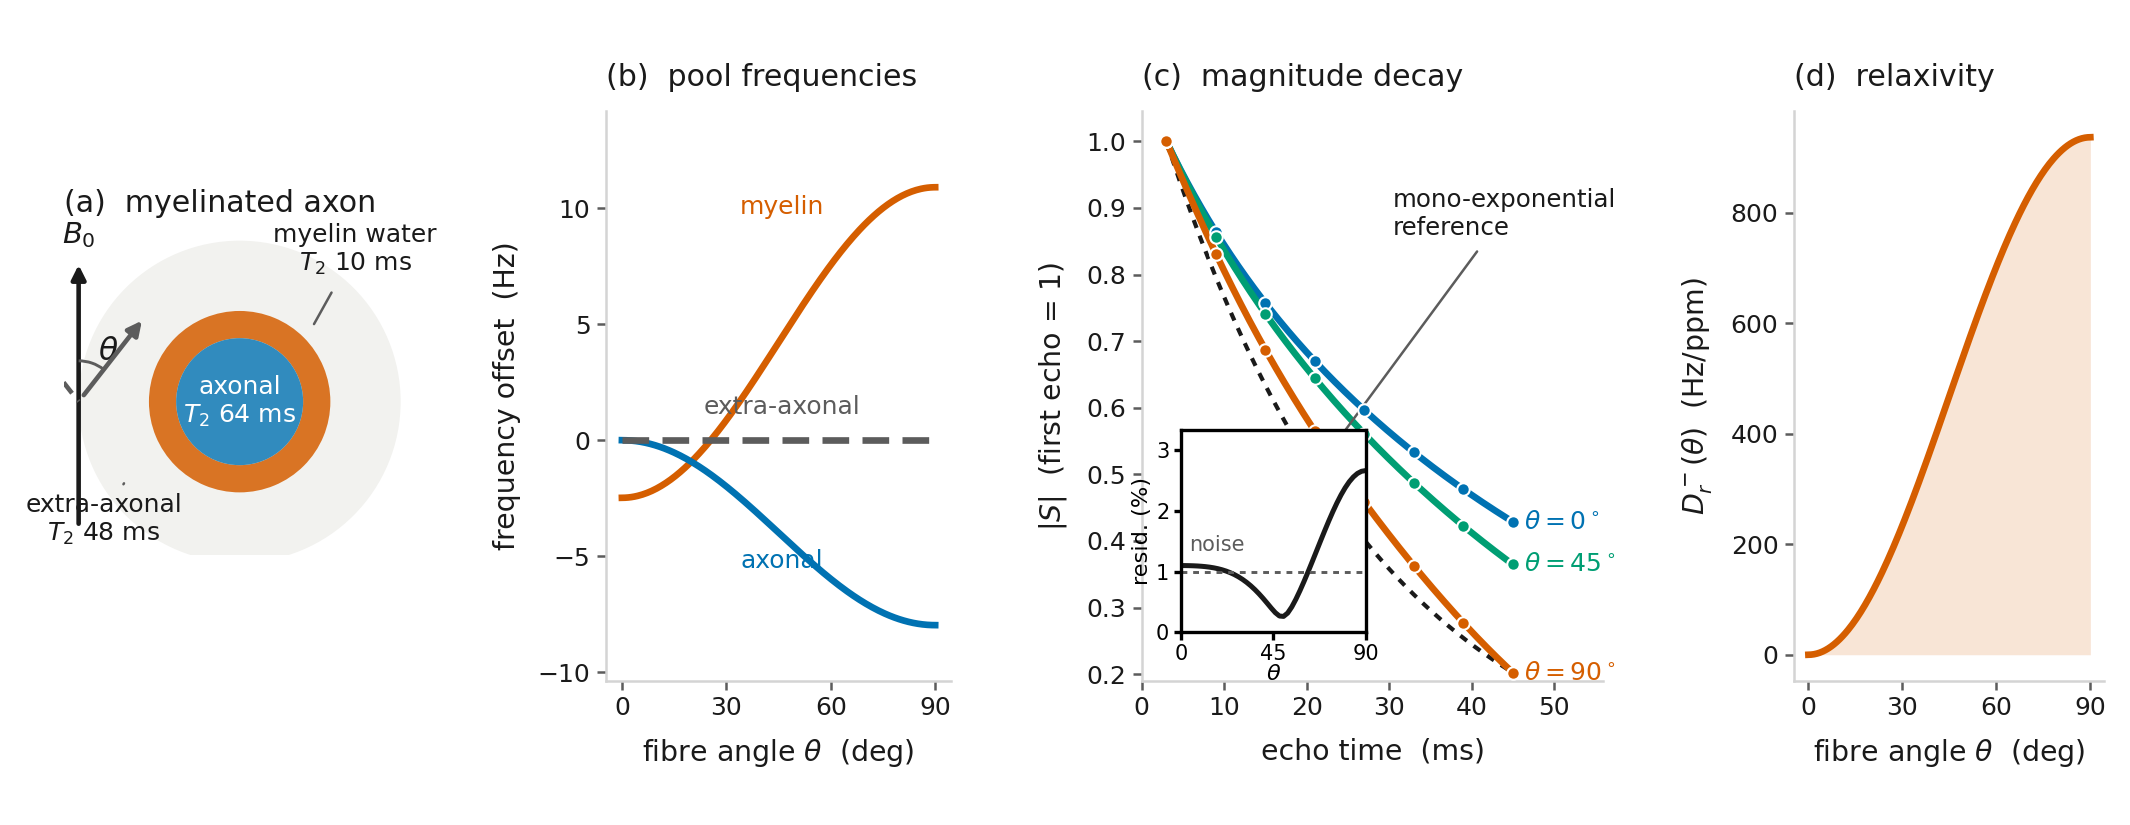
\includegraphics[width=\textwidth]{figures/fig1_concept}
\caption{The orientation of a white-matter fibre relative to $B_0$ has two observable consequences; existing source-separation methods contend with one of them and cannot see the other. (a) A myelinated axon holds water in three places, and the anisotropic, radially oriented susceptibility of the sheath places them at different Larmor frequencies. (b) Those offsets are functions of the fibre angle (Eqs.~\eqref{eq:dfa}--\eqref{eq:dfe}); the extra-axonal pool sits at zero by construction, so it is the \emph{spread} between the curves that grows with $\theta$. (c) The pools therefore interfere, and the multi-echo magnitude departs from a mono-exponential decay in a way that depends on $\theta$ and on the myelin water fraction (curves at $\mathrm{MWF}=0.12$, 7\,T, the 8-echo train used here; markers are the sampled echoes). Inset: the RMS of that departure against fibre angle, with the per-voxel noise floor at SNR 100 shaded---at large angles the effect clears the floor, near $45^\circ$ it does not, and near $\theta=0$ what remains is multi-exponential $T_2$ curvature carrying no orientation information. (d) The same angle sets the diamagnetic relaxivity, $D_r^{-}(\theta)\propto\sin^{2}\theta$, which is what leaves $\chi$-separation under-determined in white matter. All curves are computed from the model of Section~\ref{sec:theory-anchor} with the constants of Table~\ref{tab:params}.}
\label{fig:concept}
\end{figure*}

\begin{figure}[t]
\centering
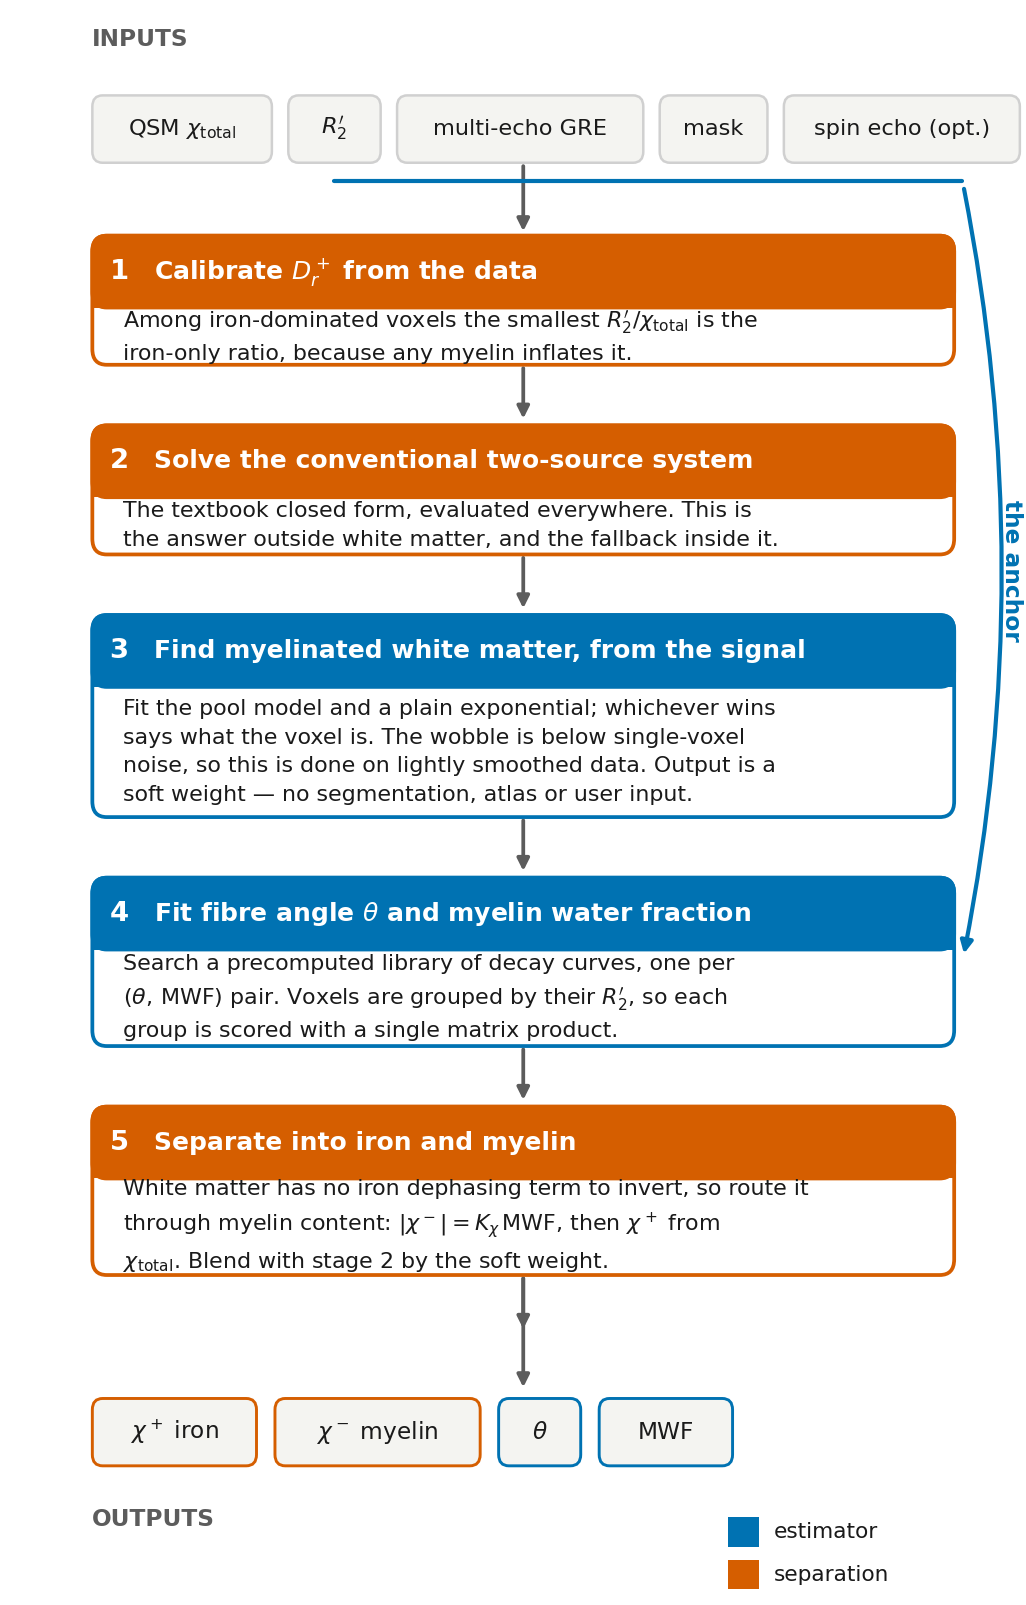
\includegraphics[width=\linewidth]{figures/fig2_pipeline}
\caption{The method end to end. Stages 3 and 4 estimate microstructure and stand independently of any separation convention; stages 1, 2 and 5 perform the separation. The anchor is the link that makes stage 4 well conditioned: the measured $R_2'$ fixes how much total decay a candidate curve must produce, leaving only the \emph{shape} of the decay to identify $\theta$ and the myelin water fraction. Nothing in the chain consumes a tissue segmentation, an atlas, a diffusion acquisition or a user decision.}
\label{fig:pipeline}
\end{figure}

\begin{figure}[t]
\figplaceholder{FIGURE 2 --- conditioning. Two side-by-side residual landscapes over $(\theta, R_2'^{\,\mathrm{meso}})$ at the true MWF, same colour scale, truth marked with a cross and grid winner with a circle. Left: unanchored, showing the long curved valley. Right: the same voxel with the $R_2'$ anchor applied, where the admissible set collapses to a curve and the minimum is isolated. \TODO{the right-hand panel does not exist yet and must be generated.}}{75mm}
\caption{Why the fit needs an anchor. Left: the residual landscape of the three-parameter fit, sliced at the true myelin water fraction, has a unique global minimum but lies in a long, shallow, curved valley in which a larger fibre angle trades against a smaller mesoscopic dephasing rate; the coarse-grid winner (circle) is far from the truth (cross) even with no noise. Right: constraining the total reversible rate to the measured $R_2'$ (Eq.~\eqref{eq:anchor}) restricts the search to a curve through the landscape, removing the ill-conditioned direction.}
\label{fig:landscape}
\end{figure}

\begin{figure}[t]
\figplaceholder{FIGURE 3 --- field dependence. (a) Mean absolute $\theta$ error against true $\theta$ at effective fields 1.27, 3.0 and 7.0\,T, SNR 100, with a horizontal line at the $\approx30^\circ$ random-guess level. (b) Mono-exponential residual RMS against $\theta$ for the same three fields with the $1/\mathrm{SNR}$ noise floors drawn as horizontal lines, showing that the residual is flat in $\theta$ at 1.27\,T and strongly $\theta$-dependent at 7\,T.}{75mm}
\caption{Orientation information in the magnitude is a strong function of field strength. (a) Fibre-angle error against true angle at three effective fields (SNR 100). At 1.27\,T the estimator is close to a random guess at every angle; at 7\,T the error is below $2^\circ$ above $35^\circ$. The residual ambiguity near $\theta=0$ is intrinsic to the $\sin^{2}\theta$ dependence and is present at every field. (b) The departure from a mono-exponential decay against the per-voxel noise floor. At 1.27\,T the departure is real but almost independent of orientation---it is multi-exponential $T_2$ curvature rather than a frequency effect---so it carries no orientation information.}
\label{fig:field}
\end{figure}

\begin{figure*}[t]
\figplaceholder{FIGURE 4 --- parameter recovery. Row 1: ground-truth $\theta$, estimated $\theta$, and error map, one axial slice, white matter only. Row 2: the same for MWF. Row 3: the soft white-matter weight $w$ with the held-out white-matter label contoured over it, plus two scatter plots ($\theta$ estimated vs true; MWF estimated vs true) with correlation and median error annotated, and the blind-fit scatter shown in grey behind the anchored one so the improvement is visible in a single panel.}{85mm}
\caption{Parameters recovered from the magnitude with $R_2'$ anchoring. Fibre angle is recovered at $r=0.862$ with a median absolute error of $8.4^\circ$, and myelin water fraction at $r=0.81$ with a median absolute error of 0.015; the corresponding unanchored values (grey, scatter panels) are $r=0.72$/$10.6^\circ$ and $r=0.29$/0.059. The soft white-matter weight, computed by model selection against a mono-exponential alternative and gated only by the input susceptibility map, agrees with the held-out white-matter label at a Dice coefficient of 0.893 despite the method receiving no segmentation.}
\label{fig:maps}
\end{figure*}

\begin{figure*}[t]
\figplaceholder{FIGURE 5 --- separation results. A grid: columns = ground truth, HC-ChiSep, closed-form null, SUSEP-Net, $\chi$-sepnet \TODO{plus the remaining comparators once re-scored}; rows = $\chi^{+}$ (axial), $\chi^{-}$ (axial), and difference from truth for each, on fixed windows stated in the caption. Add one sagittal $\chi^{-}$ row, since white matter is where the method acts and sagittal shows the corpus callosum with a full range of fibre angles.}{95mm}
\caption{Source separation on the multi-compartment phantom. Windows: $\chi^{+}\in[0,0.1]$\,ppm, $\chi^{-}\in[0,0.1]$\,ppm, difference $\pm$\NUM{0.05}\,ppm. The improvement over the closed-form null solution is concentrated in white matter and in the diamagnetic channel, as the mechanism predicts: the null must attribute all of white matter's reversible relaxation to a single scalar relaxivity, whereas HC-ChiSep resolves the orientation dependence. \TODO{point out one or two specific anatomical locations once the figure exists---the corpus callosum genu/splenium contrast and an internal-capsule region would make the point concretely.}}
\label{fig:sep}
\end{figure*}

\begin{figure*}[t]
\figplaceholder{FIGURE 6 --- in vivo. \TODO{Suggested layout: row 1, input $\chi_{\mathrm{total}}$ and $R_2'$; row 2, HC-ChiSep $\chi^{+}$ and $\chi^{-}$ beside a comparator method; row 3, estimated $\theta$ and MWF maps with the DTI-derived fibre angle beside them where available, plus a scatter. If a repositioned-head or scan--rescan acquisition exists, add a difference panel.}}{90mm}
\caption{\TODO{In vivo caption. It should state the field strength and protocol in the first sentence, name what the reader should look at, and be explicit that no ground truth exists so the panels are qualitative except where a DTI or myelin-water-imaging reference is shown.}}
\label{fig:invivo}
\end{figure*}

\bibliography{hc-chisep}

\vfill\pagebreak

\end{document}
